\documentclass[12]{article}
\usepackage{titlesec}
\usepackage{indentfirst}
\usepackage [english]{babel}
\usepackage [utf8]{inputenc}
\usepackage [T1] {fontenc}
\usepackage{subfiles}
\usepackage{wrapfig}
\usepackage{graphicx}
\usepackage{sidecap}
\usepackage{amssymb}
\usepackage{amsmath}
\usepackage{multirow}
\usepackage[english]{babel}
\graphicspath{ {./images/} }
\usepackage[export]{adjustbox}
\usepackage{enumitem}
\usepackage[absolute,overlay]{textpos}
\usepackage{float}
\usepackage{forest}
\usepackage{amsmath,amsfonts,amsthm,amssymb}
\usepackage{graphicx}
\usepackage{pdfpages}
\usepackage{amsmath}
\addtocontents{toc}{\protect\thispagestyle{empty}}
\usepackage[margin = 2.8 cm, headheight = 1.5pt]{geometry}
\usepackage{hyperref}
\usepackage{graphicx}

\usepackage{colortbl}
\usepackage{textgreek}

\begin{document}

\newpage
\section{Object-to-gateway communication via Bluetooth}



\subsection{Bluetooth analysis}

Here we analyze the Bluetooth signal between 2 devices, a phone and a computer. In our case the computer is the transmitter (the master, and the phone the active slave). We transfer a 4.88 MB (39.04 Mb) file over several distances and several times in order to find an average time, then the throughput in Mbps. We can clearly see that the signal throughput decreases as the distance increases.

\begin{table}[H]
\centering
\begin{tabular}{|l|l|l|l|l|l|l|}
\hline
\rowcolor[HTML]{000000}
{\color[HTML]{FFFFFF} \textbf{Distance}} & {\color[HTML]{FFFFFF} \textbf{Measurement 1}} & {\color[HTML]{FFFFFF} \textbf{Measurement 2}} & \multicolumn{1}{c|}{\cellcolor[HTML]{000000}{\color[HTML]{FFFFFF} \textbf{M. 3}}} & {\color[HTML]{FFFFFF} \textbf{M. 4}} & {\color[HTML]{FFFFFF} \textbf{Average}} & {\color[HTML]{FFFFFF} \textbf{Throughput (kbps)}} \\ \hline
1m                                       & 50s                                      & 56s                                      & 53s                                                                                   & 53s                                      & 53s                                     & 736.6                                       \\ \hline
2m                                       & 55s                                      & 61s                                      & 60s                                                                                   & 58s                                      & 58.5s                                   & 667.4                                       \\ \hline
3m                                       & 55s                                      & 60s                                      & 64s                                                                                   & 59s                                      & 59.5s                                   & 656.1                                       \\ \hline
4m                                       & 72s                                      & 67s                                      & 73s                                                                                   & 70s                                      & 70.5s                                   & 553.7                                       \\ \hline
5m                                       & 75s                                      & 78s                                      & 79s                                                                                   & 77s                                      & 77.25s                                  & 505.0                                       \\ \hline
\end{tabular}
\end{table}


\begin{figure}[H]
    \centering
    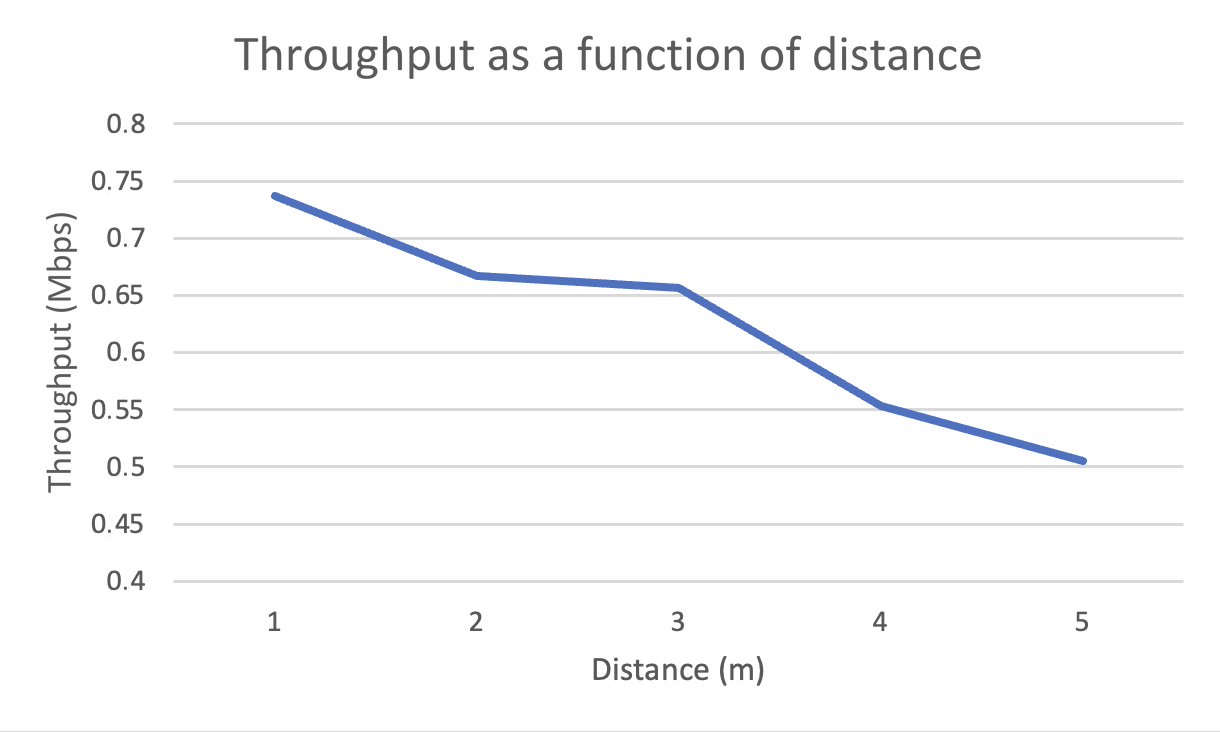
\includegraphics[width=0.7\linewidth]{Capture d’écran 2024-03-08 à 11.37.05.png}
    \caption{Graph of throughput as a function of distance}
    \label{fig:enter-label}
\end{figure}

\newpage
\subsection{Bluetooth network architecture}

Next, we measured the average transfer speed between a gateway and a device located at a distance of 3 meters; we obtain a measurement of 656.1 Kbps at 3 meters.\\

Knowing that each gateway must have a minimum throughput of 100 Kbps, a gateway can therefore manage a maximum of 6 objects. We also know that each group of objects must necessarily contain one master and a defined number of slaves. We therefore have 6 objects for 5 gateways and 5 for one gateway $ \frac{35}{6} = 5.89 \approx 6$.\\

We must place our different objects in an area of 20 m by 20 m; in order to maximize the range and limit network interference, we arranged them in the following way, as shown in \textit{Figure 2}.


\begin{figure}[H]
    \centering
    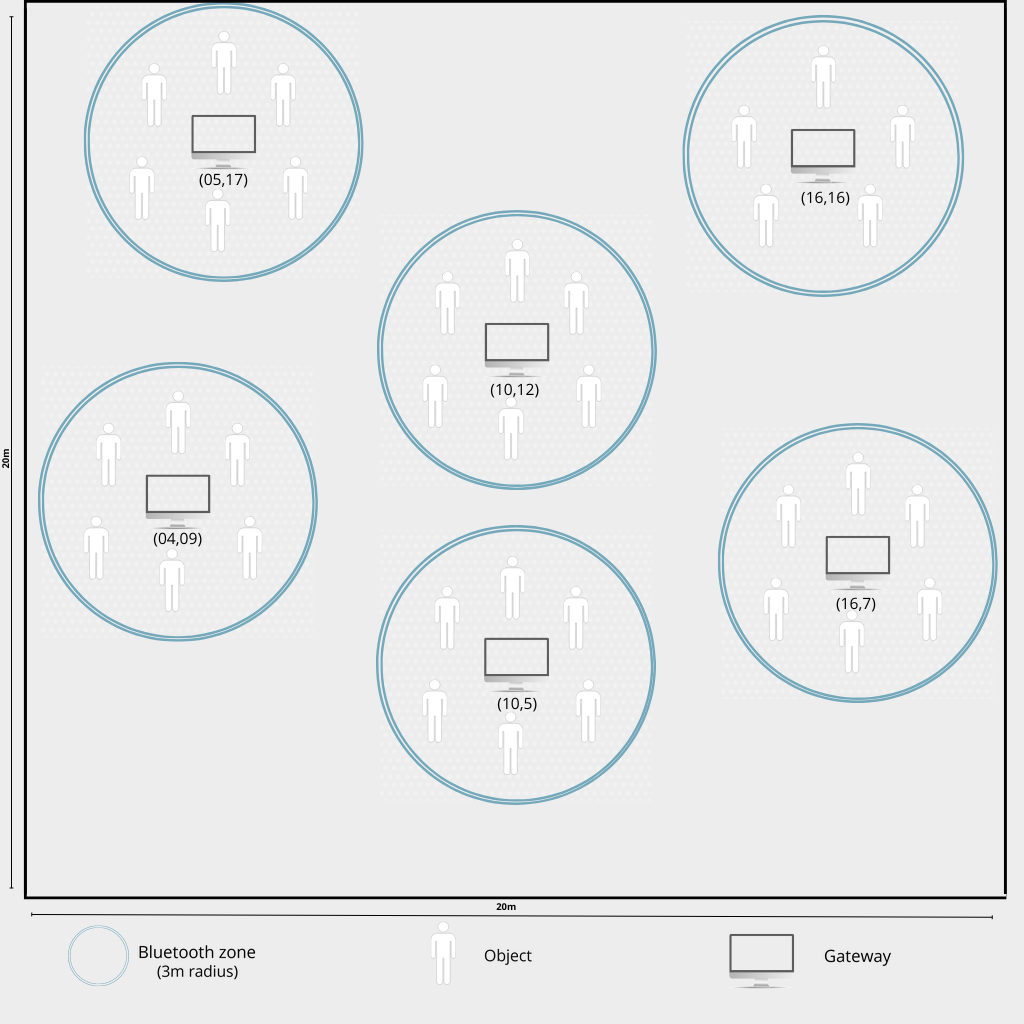
\includegraphics[width=1\linewidth]{Votre texte de paragraphe (2).png}
    \caption{Diagram of the Bluetooth network architecture}
    \label{fig:enter-label}
\end{figure}


\subsection{Reduced transmission power}

We now look for the transmission power of the Bluetooth. We have a throughput of 653.9 Kb/s at 3 meters.
A gateway must be able to provide a throughput of at least 100 Kbps per object while only being able to manage 7 of them. We will therefore need 5 masters managing 6 slaves and one last master managing only 5 slaves to obtain the right count of 35 active objects while respecting the throughput required for each object.\\


Next, we are looking for the reduced transmission power of the Bluetooth module in order to determine the power class to which the module belongs. First, the calculation of the SINR (signal to interference plus noise ratio) is necessary with the data obtained previously.


\begin{equation*}
    \text{SINR} = 2^{\frac{D}{B}} - 1 =  2^{\frac{656.1}{1000}} - 1 = 0.58
\end{equation*}

We then look for the thermal noise power of the Bluetooth.

\begin{equation*}
    P_b = K \times T \times B = 1.38.10^{-23} \times 290 \times 10^9 = 4.10^{-12} \text{ mW}
\end{equation*}

Now, we have the interference power $P_i = -90$ dBm. Which, once converted into mW, is $10^{-9}$ mW. We can then calculate the received power.\\

\begin{equation*}
    P_r = \text{SINR} \left( P_b + P_i \right)
\end{equation*}

\begin{equation*}
    0.58 \left( 4.10^{-12} + 10^{-9} \right) = 5.8232.10^{-10} \text{ mW}
\end{equation*}
\\

We know that the formula to calculate the transmitted power requires the knowledge of two terms. First the received power (Pr), which we obtained previously with a value of $P_r = 5.8232.10^{-10}$, then secondly the attenuation coefficient, which obeys the following formula: $A_{EL} = 32.4 + 20 \log_{10} \left( d \right) + 20 \log_{10} \left( f \right) $ where d = 3m ($3.10^{-3}$) and f = 2.4 GHz (2400 Hz).

\begin{equation*}
    A_{EL} = 32.4 + 20 \log_{10} \left( 3.10^{-3} \right) + 20 \log_{10} \left( 2.4.10^{3} \right)
\end{equation*}

\begin{equation*}
    A_{EL} = 49.5 \text{ dBm}
\end{equation*}

After obtaining these two terms we can move on to the calculation of the transmitted power, which is calculated by multiplying the received power by the attenuation coefficient converted into milliwatts since we had it in dBm.

\begin{equation*}
    P_{e} = P_{r} \times A
\end{equation*}

\begin{equation*}
    P_{e} = 5.8232.10^{-10} \times 10^{4.95}
\end{equation*}

\begin{equation*}
    P_{e} = 5.19.10^{-5} \text{ mW}
\end{equation*}

We are then in Bluetooth power class 3 since we have a transmission power value below 0.8 mW.

\section{Gateway-to-central-server communication via Wi-Fi}

\subsection{Determining the number of required access points}

In this part, we want to calculate the number of access points needed to cover the studied surface. \\

We start with the calculation of the average RSSI on the ISEP EAP network.

\begin{table}[H]
\centering
\begin{tabular}{|l|l|l|l|l|}
\hline
\rowcolor[HTML]{000000}
{\color[HTML]{FFFFFF} Measurement} & {\color[HTML]{FFFFFF} 1} & {\color[HTML]{FFFFFF} 2} & {\color[HTML]{FFFFFF} 3} & {\color[HTML]{FFFFFF} 4} \\ \hline
RSSI (dBm) & -57 & -59 & -55 & -56 \\ \hline
RSSI (mW) & $2.0 \times 10^{-6}$ & $1.2 \times 10^{-6}$ & $3.1 \times 10^{-6}$ & $2.5 \times 10^{-6}$ \\ \hline
\end{tabular}
\end{table}

We calculate the average of these values:

\begin{equation*}
\text{Avg}_\text{RSSI} = \frac{57 + 59 + 55 + 56}{4} = 56.75\text{ dBm}
\end{equation*}

The average received signal power is 56.75dBm. \\

From this value, we will look for the maximum range corresponding to a throughput of 250Mb/s.

We calculate the value of the attenuation:
\begin{equation*}
    \text{A}= \text{EIRP}+\text{RSSI}= 5 + 56.75 = 61.75dBm
\end{equation*}

We take the attenuation coefficient formula
\begin{equation*}
    \text{A} = 32.4 + 20 \log_{10}(d_\text{km}) + 20 \log_{10}(f_\text{MHz}) + 35 \log_{10} \left( \frac{d_m}{ds_m} \right)
\end{equation*}

From the second formula, we can deduce that:

\begin{equation*}
    55 \log_{10} \left( d_m \right) = \text{A} - 32.4 - 20 \log_{10}(f_\text{GHz}) + 35 \log_{10} \left( ds_m \right)
\end{equation*}

We take:

\begin{equation*}
    res = \text{A} - 32.4 - 20 \log_{10}(f_\text{GHz}) + 35 \log_{10} \left( ds_m \right)
\end{equation*}

\begin{equation*}
    res = 61.75 - 32.4 - 20 \log_{10}(f_\text{GHz}) + 35 \log_{10} \left( ds_m \right)
\end{equation*}

\begin{equation*}
    res = 46.20
\end{equation*}

And we can isolate the distance:

\begin{equation*}
    \text{d}_\text{m} = 10^{\frac{46.20}{55}} = 6.91 \text{m}
\end{equation*}

The maximum range corresponding to a throughput of 250Mb/s is 6.91m \\

We now look for the number of access points needed (N) to cover a surface of 400m². For this, we use the surface covered by one access point:

\begin{equation*}
    \text{N} = \frac{400}{\pi \times 6.91^2} = 2.67
\end{equation*}

To cover a surface of $400 \text{m}^2$ in our configuration, 3 access points are needed.

\subsection{Wi-Fi network architecture}

Thanks to the calculations carried out previously, we found that each Wi-Fi access point covered a circle-shaped area with a radius of 6.91m. After several positioning attempts, we saw that the whole network can be covered with only two Wi-Fi access points, which makes it possible to lighten the network and make it less expensive. We therefore obtain the following figure:
\begin{figure}[H]
    \centering
    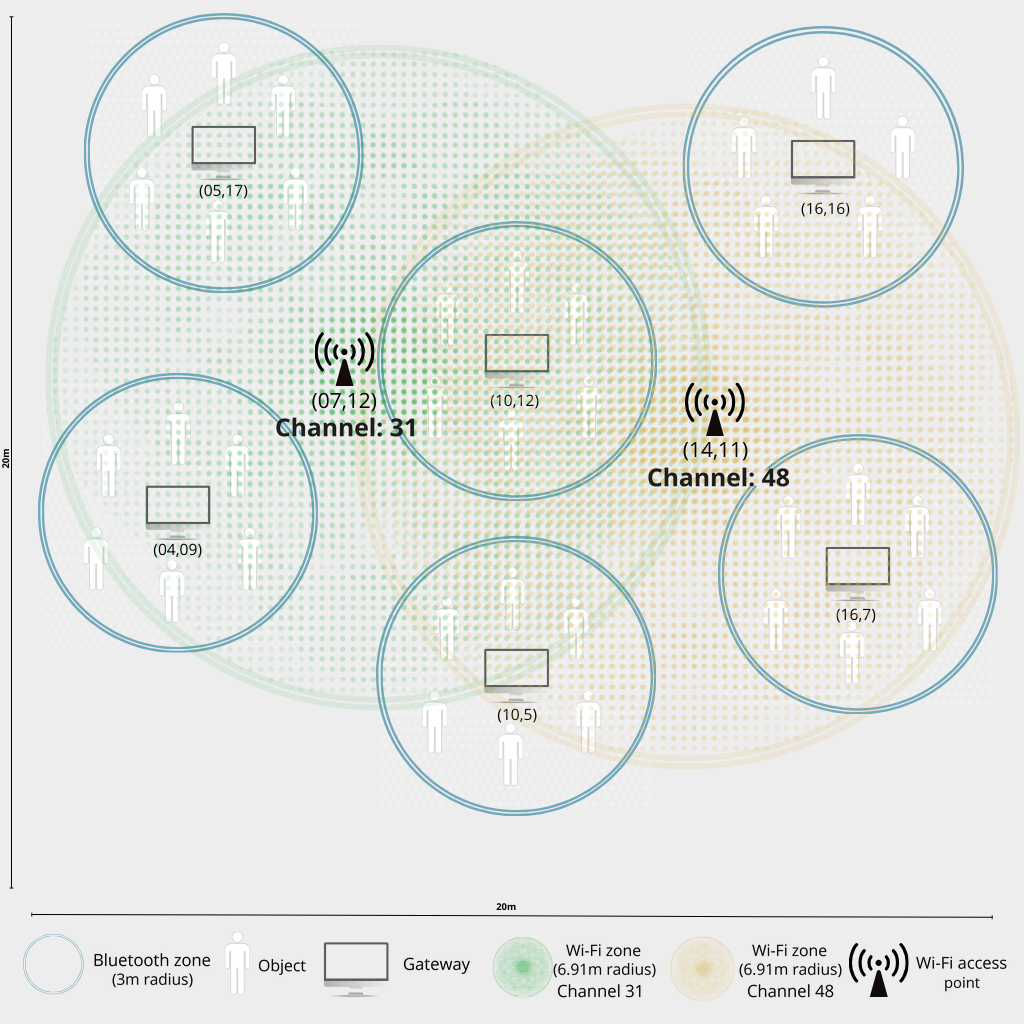
\includegraphics[width=1\linewidth]{Votre texte de paragraphe (3).png}
    \caption{Diagram of the network architecture (Bluetooth and WiFi)}
    \label{fig:enter-label}
\end{figure}



\subsection{Access point planning}

\subsubsection{Measurements}

\begin{table}[H]
\resizebox{\textwidth}{!}{%
\begin{tabular}{|l|l|l|c|c|c|c|}
\hline
\rowcolor[HTML]{000000}
{\color[HTML]{FFFFFF} Location} & \multicolumn{1}{c|}{\cellcolor[HTML]{000000}{\color[HTML]{FFFFFF} SSID}} & \multicolumn{1}{c|}{\cellcolor[HTML]{000000}{\color[HTML]{FFFFFF} MAC address}} & \multicolumn{1}{l|}{\cellcolor[HTML]{000000}{\color[HTML]{FFFFFF} Carrier frequency}} & \multicolumn{1}{l|}{\cellcolor[HTML]{000000}{\color[HTML]{FFFFFF} Channel}} & \multicolumn{1}{l|}{\cellcolor[HTML]{000000}{\color[HTML]{FFFFFF} Bandwidth}} & \multicolumn{1}{l|}{\cellcolor[HTML]{000000}{\color[HTML]{FFFFFF} Wi-Fi version}} \\ \hline
\cellcolor[HTML]{000000}{\color[HTML]{FFFFFF} \begin{tabular}[c]{@{}l@{}}Third floor\\ corridor\end{tabular}} & ISEP EAP & c0:c7:0a:98:f2:c1 & 5 GHz & 64 & 80 MHz & 802.11ax \\ \hline
\cellcolor[HTML]{000000}{\color[HTML]{FFFFFF} \begin{tabular}[c]{@{}l@{}}Staircase between \\ floors 1 and 2\end{tabular}} & ISEP EAP & c0:c7:0a:9c:02:91 & 5 GHz & 120 & 80 MHz & 802.11ax \\ \hline
\cellcolor[HTML]{000000}{\color[HTML]{FFFFFF} \begin{tabular}[c]{@{}l@{}}Outside ISEP\\ entrance side\end{tabular}} & ISEP EAP & c0:c7:0a:9c:05:01 & 5 GHz & 108 & 80 MHz & 802.11ax \\ \hline
\cellcolor[HTML]{000000}{\color[HTML]{FFFFFF} \begin{tabular}[c]{@{}l@{}}Outside ISEP\\ park side\end{tabular}} & ISEP EAP & c0:c7:0a:9d:17:31 & 5 GHz & 128 & 80 MHz & 802.11ax \\ \hline
\cellcolor[HTML]{000000}{\color[HTML]{FFFFFF} Common room} & ISEP EAP & c0:c7:0a:5c:36:91 & 2.4 GHz & 7 & 40 MHz & 802.11n \\ \hline
\end{tabular}%
}
\end{table}

\subsubsection{Analysis}

Following this operation, it was observed that the network name (SSID) remains the only constant, while the Wi-Fi bandwidth and the Wi-Fi version vary according to the frequency used. It was also noted that the ISEP Wi-Fi access points are not uniformly set to the same channel, favoring the use of distinct channels for each access point within the same area; this was put in place in order to minimize interference. Indeed, each access point operates on a different channel, with a preference for a 5GHz carrier frequency.




\section{Comparison of Wi-Fi and Bluetooth with alternative technologies}

Here are five short-range wireless technologies that are alternatives to Wi-Fi and Bluetooth:

1. Z-Wave
2. NFC (Near Field Communication)
3. Zigbee
4. LoRa (Long Range)
5. Infrared

Here is a comparative table based on the requested criteria:

\begin{center}
\begin{tabular}{|c|c|c|c|c|c|}
\hline
 &  &  &  & Simultaneous &  \\
Technology & Bandwidth & Throughput & Range & Connections & Cost \\
\hline
Wi-Fi & Wide & High & Medium/Long & High & Moderate to High \\
Bluetooth & Narrow & Low to Medium & Short/Medium & Moderate & Low to Moderate \\
Z-Wave & Narrow & Low & Medium/Long & High & Moderate to High \\
NFC & Very Narrow & Very Low & Very Short & Low & Low \\
Zigbee & Narrow & Low to Medium & Short/Medium & High & Moderate \\
LoRa & Wide & Low to Medium & Long & High & Moderate \\
Infrared & N/A & Low & Short & Low & Low \\
\hline
\end{tabular}
\end{center}


Conclusions on the relevance of choosing the Wi-Fi and Bluetooth technologies:
\begin{itemize}
    \item Wi-Fi: Offers a wide bandwidth, a high throughput and a medium to long range, which makes it a relevant choice for applications requiring high-speed data transmission over long distances, such as home and professional networks.
    \item Bluetooth: With a narrow bandwidth, a variable throughput, a short to medium range and a moderate number of simultaneous connections, Bluetooth is better suited to applications requiring low energy consumption and connectivity between devices over short distances, such as wireless earphones and personal IoT devices.
\end{itemize}





\end{document}
